\documentclass[a4paper,12pt]{report}
\usepackage{float, amsmath, bm, graphicx, numprint, multicol, caption}

\begin{document}

\setlength{\abovedisplayskip}{6pt}
\setlength{\belowdisplayskip}{8pt}
\setlength{\abovedisplayshortskip}{2pt}
\setlength{\belowdisplayshortskip}{8pt}

\title{Project 3 Report}
\author{Dylan Callaway}
\date{Engineering 150 \\ Fall 2019}
\maketitle

\pagenumbering{roman}
\tableofcontents
\newpage
\pagenumbering{arabic}

\newenvironment{nscenter}
 {\setlength{\topsep}{0ex}\trivlist\item\relax\centering}
 {\endtrivlist}

\section{Introduction}
The scenario being modeled in this project is that of a robotic 3D printer arm. A dispenser at the end of the arm extrudes electrically charged droplets above a substrate. The droplets then fall and land on the substrate, which in some cases may also be charged in certain areas, forming a pattern.

The path the arm and the dispenser take, which ultimately determines the droplet pattern, is set by the angular velocities of the arm linkages. Furthermore, the dispenser imparts some force on the droplets as they are extruded which increases their velocity relative to the dispenser when they are released.The angular velocities and the additional extrusion velocity are parameters of the arm specified by the user, and can be set to produce specific patterns.

This paper introduces the physical laws governing the motion of the printer arm and droplets, describes the rendering of the physical laws into a numerical simulation, and demonstrates the effectiveness of a genetic algorithm in determining angular velocities and additional extrusion velocity necessary to produce a predetermined pattern of droplets.


\section{Background and Theory}
The dynamics of the printer arm and dispenser are governed by the arm geometry and the angular velocity of each linkage $\dot{\Theta}_i$, where $i \in \{1, 2, 3\}$.
\begin{figure}[H]
\begin{nscenter}
  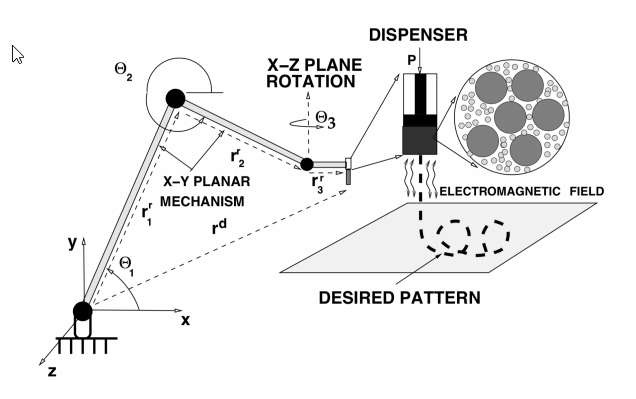
\includegraphics[width=0.75\linewidth]{arm_geom.png}
  \caption[test]{3D Printer Arm Geometry Diagram.\footnotemark}
  \end{nscenter}
\end{figure}
\footnotetext{Credit E150 Assignment 3, T. Zohdi, UC Berkeley.}\noindent
Given linkage lengths $L_i = \{0.3, 0.2, 0.08\}$, the dispenser position $r_d$ can be solved for as a function of $\Theta_i$:
$$ \bm{r}_d =
\begin{bmatrix}
x_d \\
y_d \\
z_d
\end{bmatrix} = 
\begin{bmatrix}
L_1\cos{\Theta_1} + L_2\cos{\Theta_2} + L_3\sin{\Theta_3} \\
L_1\sin{\Theta_1} + L_2\sin{\Theta_2}\\
L_3\cos{\Theta_3}
\end{bmatrix} $$
Taking the time derivative of the dispenser position produces the dispenser velocity as a function of $\Theta_i$ and $\dot{\Theta}_i$:
$$ \bm{v}_d = \dot{\bm{r}}_d =
\begin{bmatrix}
\dot{x_d} \\
\dot{y_d} \\
\dot{z_d}
\end{bmatrix} = 
\begin{bmatrix}
-L_1\dot{\Theta}_1\sin{\Theta_1} - L_2\dot{\Theta}_2\sin{\Theta_2} + L_3\dot{\Theta}_3\cos{\Theta_3} \\
L_1\dot{\Theta}_1\cos{\Theta_1} + L_2\dot{\Theta}_2\cos{\Theta_2} \\
-L_3\dot{\Theta}_3\sin{\Theta_3}
\end{bmatrix}
$$
The initial position and velocity of each droplet, $\bm{r}_e^0$ and $\bm{v}_e^0$, respectively, are determined by the state of the dispenser at that time, as well as the additional extrusion velocity $\Delta \bm{v}^d$ such that:
$$ \bm{r}_e^0 = \bm{r}_d \qquad \bm{v}_e^0 = \bm{v}_d + \Delta \bm{v}^d  $$
Once the droplets have been extruded, there are three forces acting on them that cause them to accelerate as they fall towards the substrate. Firstly, gravity accelerates the droplets in the $-Y$ direction at a rate of $9.81\frac{m}{s^2}$. Secondly, the point charges on the substrate, at positions $r_p$, interact with the charged droplets\footnote{The electrical interaction between droplets is ignored.}, accelerating them according to:
$$ \bm{a}_e^{elec} = \frac{1}{m_e}\sum_{p=1}^{N_c} \frac{q_pq_e}{4\pi\epsilon||\bm{r}_e-\bm{r}_p||^2}(\bm{r}_e - \bm{r}_p) $$
where $m_e$ is the mass of the individual droplets, $q_p$ is the charge of the points on the substrate, $q_e$ is the charge of the droplets, and $\epsilon$ is the electrical permittivity of free space. Each of the droplets is made up of two distinct phases with density $\rho_1$ and $\rho_2$ and charge capacity $q_1$ and $q_2$. The volume fraction, $v_2$, of the second phase and the overall droplet volume, $V_e$, are determined by the dispenser and allow the overall droplet mass and charge to be determined according to:
$$ m_e = V_e((1-v_2)\rho_1 + v_2\rho_2) \qquad q_e = V_e((1-v_2)q_1 + v_2q_2) $$
Finally, as the printer arm is assumed to be operating near sea level, the drag force accelerates the droplets in the direction opposite to their velocity, defined as:
$$ \bm{a}_e^{drag} = \frac{1}{2m_e}\rho_aC_{De}A_e^D||\bm{v}^f - \bm{v}_e||(\bm{v}^f - \bm{v}_e)$$
where $\rho_a$ and $v^f$ are the density and velocity of the surrounding air, $A_e^D$ is the cross-sectional area of the droplets, which are assumed to be spherical, and $C_{De}$ is the drag coefficient of the droplets, defined as a function of the Reynolds number of the droplets as follows:
$$C_{De}=
\begin{cases}
\frac{24}{Re}, & 0 < Re \leq 1 \\
\frac{24}{Re^{0.0646}}, & 1 < Re \leq 400 \\
0.5, & 400 < Re \leq 3\times10^5 \\ 
0.000366Re^{.4275}, & 3\times10^5 < Re \leq 2 \times 10^6 \\
0.18, & Re > 2 \times 10^6
\end{cases}
, \quad Re = \frac{2R\rho_a||\bm{v}^f - \bm{v}_i||}{\mu_f}
$$
where $R$ is the droplet's radius and $\mu_f$ is the viscosity of the surrounding air.
These three accelerations are then summed to produce the total acceleration on each droplet, $\bm{a}_e$.


\section{Procedure and Methods}
The above equations fully describe the printer arm and droplets as a system of differential equations where:
$$ \Theta_i(t) = \Theta_i^0 + \dot{\Theta}_i t \qquad \bm{r}_e(t) = \bm{r}_e^0 + \int_{0}^{t}\bm{v}_e(t) dt \qquad \bm{v}_e(t) = \bm{v}_e^0 + \int_{0}^{t}\bm{a}_e(t) dt$$
Because the angular velocities of the linkages are constant, their angular position can be determined according to:
$$ \Theta_i(t) = \Theta_i^0 + \dot{\Theta}_it $$
and the  equations describing the droplets after extrusion can be solved in discrete time using the Forward Euler Method such that:
$$ \bm{r}_e(t+\Delta t) = \bm{r}_e(t) + \Delta t \bm{v}_e(t) \qquad \bm{v}_e(t+\Delta t) = \bm{v}_e(t) + \Delta t \bm{a}_e(t) $$
The dispenser extrudes a new droplet every $\Delta t = 0.001s$ for $T = 3s$ total and the simulation is continued until all of the extruded droplets have landed ($y_e=0$).

These equations are then solved numerically under various conditions using MATLAB. First, the complete physical model is implemented and final droplet pattern determined for $\dot{\Theta}_1=0.2$,  $\dot{\Theta}_2=-0.2$, $\dot{\Theta}_3 = 10$ and $\Delta\bm{v}^d = [0, -1.2, 0]$. Second, the acceleration due to the electrical forces is removed, and this new droplet pattern is compared to that from the full model. Finally, the electrical and aerodynamic drag forces are removed, such that the droplets only experience a constant downward acceleration due to gravity. This enables the droplet pattern to be solved for analytically by integrating the position of the droplets twice:
$$ \bm{r}_e(t_{final}) = \int_{0}^{t_{final}}\int_{0}^{t_{final}}\bm{a}_e dt dt = \int_{0}^{t_{final}}\bm{a}_e(t_{final}) + \bm{v}_e dt$$
performing the final integration yields the desired equation used in the simplified model:
$$ \bm{r}_e(t_{final})= \bm{r}_e^0 + \bm{v}_e t_{final} + \frac{1}{2}\bm{a}_e t_{final}^2 $$
where $t_{final}$ is the time at which $y_e=0$.


\section{Results and Discussion}
\subsection{Complete Physical Model}
After the numerical and analytical solutions described above are complete, they are plotted in a variety of ways to demonstrate the differing behavior of the droplets in each respective model.
\begin{figure}[H]
\begin{nscenter}
  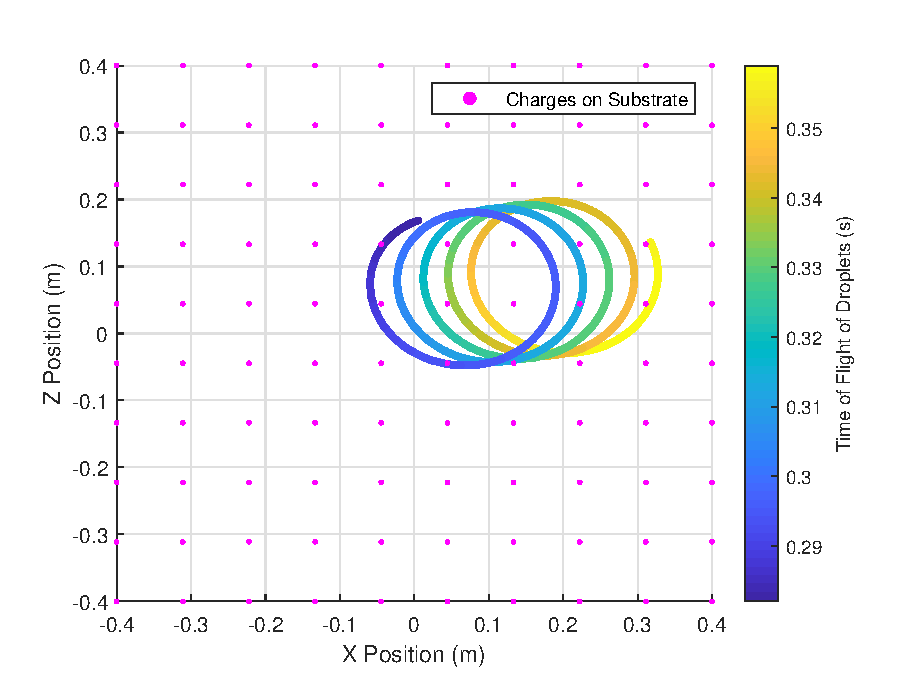
\includegraphics[width=0.75\linewidth]{part1_2.eps}
  \caption{Droplet pattern produced by complete physical model with TOF (time of flight) shown in colorbar.}
  \end{nscenter}
\end{figure}
\begin{figure}[H]
\begin{nscenter}
  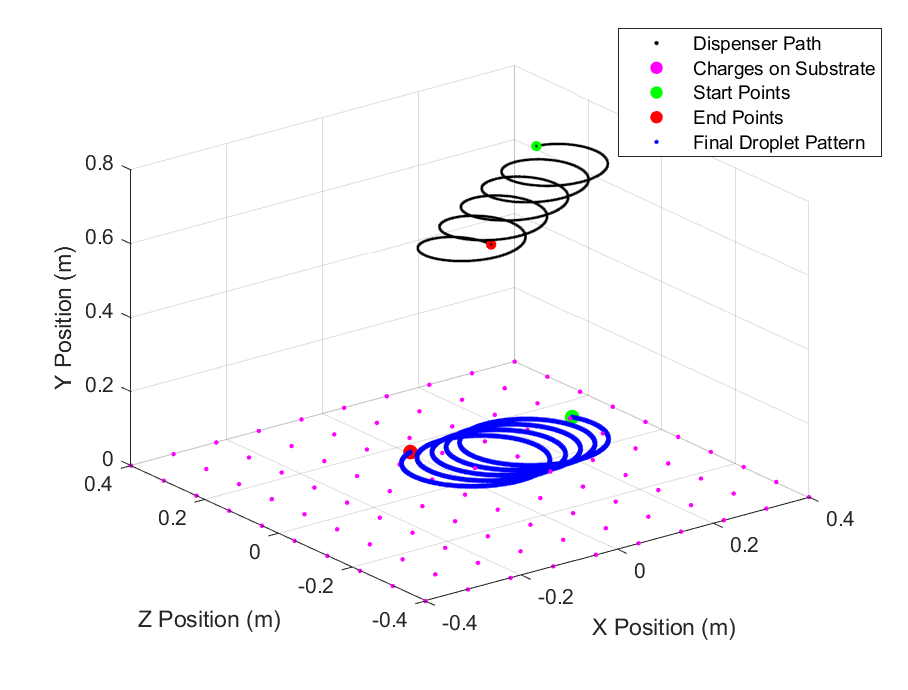
\includegraphics[width=0.75\linewidth]{part1_3.eps}
  \caption{Droplet pattern produced by complete physical model with dispenser path, start, and end points shown.}
  \end{nscenter}
\end{figure}
The path taken by the dispenser on this printer arm is limited to circles of varying position. This is because the third linkage is of a fixed length and only rotates in the $x-z$ plane. This fact, along with the aerodynamic drag and electric forces produce a pattern of slightly warped circles with translating center point. The center point position depends on the position of the end of linkage two.
\begin{figure}[H]
\begin{nscenter}
  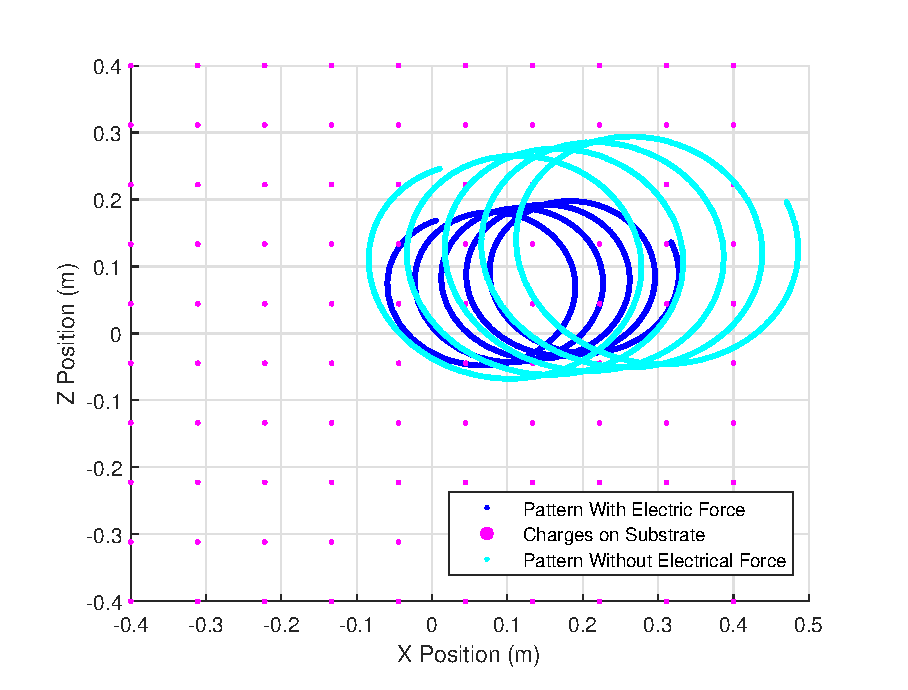
\includegraphics[width=0.75\linewidth]{part1_5.eps}
  \caption{Droplet pattern produced by physical model with and without electrical force.}
  \end{nscenter}
\end{figure}
With the electrical forces removed, the radius of the circles in the droplet pattern increases significantly. This occurs for two primary reasons.

First, because the droplets and grid of point charges are oppositely charged, the droplets are accelerated more quickly to the substrate with the electrical forces in place. Opposite to the force of aerodynamic drag, this reduces the amount of time they have to travel outward from the center point of the dispenser. We know the droplets are moving outward when they are extruded because the tangential component of the velocity of the dispenser is maintained when the droplet is released, however the radial component of the acceleration is not.

Furthermore, the grid of point charges acts as a damper to the motion of the droplets, further limiting their expansion as they move downward. It is intuit to visualize this by imagining a bowl with a ball in it. A droplet within a grid of four point charges will need to overcome the magnetic potential (sides of the bowl) at each corner of the grid before being able to move to another grid, and if it cannot it will remain within that original grid.


\subsection{Simplified Free Fall Model with Optimization}
To further simplify the model of the system such that it can be efficiently optimized to produce a desired pattern, the aerodynamic drag forces are removed along with the electrical forces. The analytical solution described earlier can then be used instead of the computationally intensive numerical solution from the simulation of the more complete model.

\begin{figure}[H]
\begin{nscenter}
  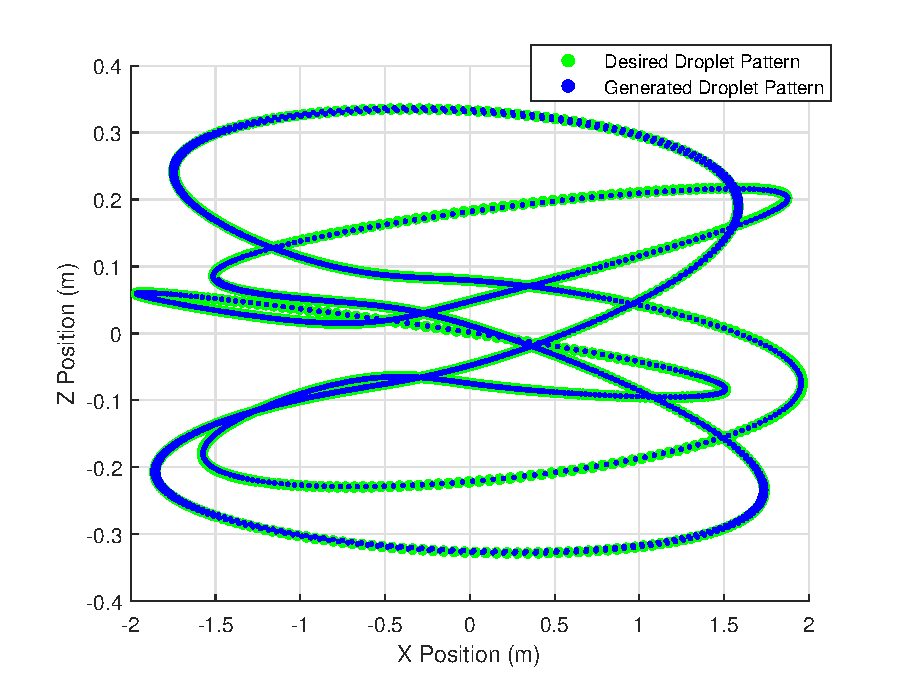
\includegraphics[width=0.75\linewidth]{part2_3.eps}
  \caption{Droplet pattern produced by optimized simplified model compared to desired droplet pattern.}
  \end{nscenter}
\end{figure}

This droplet pattern was produced with Design 1 from Table 1, where $\Lambda_1 = \dot{\Theta}_1$, $\Lambda_2 = \dot{\Theta}_2$, $\Lambda_3 = \dot{\Theta}_3$, and $\Lambda_4 = \Delta v^d_y$. $\Pi$ is the cost function used in the optimization and is defined as:
$$ \Pi = \frac{\sum_{e=1}^{N_d}||\bm{r}_e^{des} - \bm{r}_e^{gen}||}{\sum_{e=1}^{N_{d-1}}||\bm{r}_e^{des} - \bm{r}_{e+1}^{des}||} $$

A genetic algorithm was used to perform the optimization on a design population of 100 across 100 generations. Ten parents were kept from the population of generation, and ten children produced each generation from the ten parents.

\begin{table}[H]
\centering
\caption{Design Parameters and Cost of Best Designs}
\resizebox{0.75\textwidth}{!}{
\begin{tabular}{c|c|c|c|c|c}
 Design & $\Pi$ & $\Lambda_1$ & $\Lambda_2$ & $\Lambda_3$ & $\Lambda_4$ \\ 
 \hline
 \hline
1 & 0.479 & 15.709 & 15.717 & 6.286 & -3.183 \\

2 & 0.479 & 15.709 & 15.717 & 6.286 & -3.183 \\

3 & 0.479 & 15.709 & 15.717 & 6.286 & -3.183 \\

4 & 0.479 & 15.709 & 15.717 & 6.286 & -3.183 \\

\end{tabular}
}
\end{table}

The best four designs are all the same in this case, which implies good convergence from the optimization. This can be seen further in Figure 6 below.

\begin{figure}[H]
\begin{nscenter}
  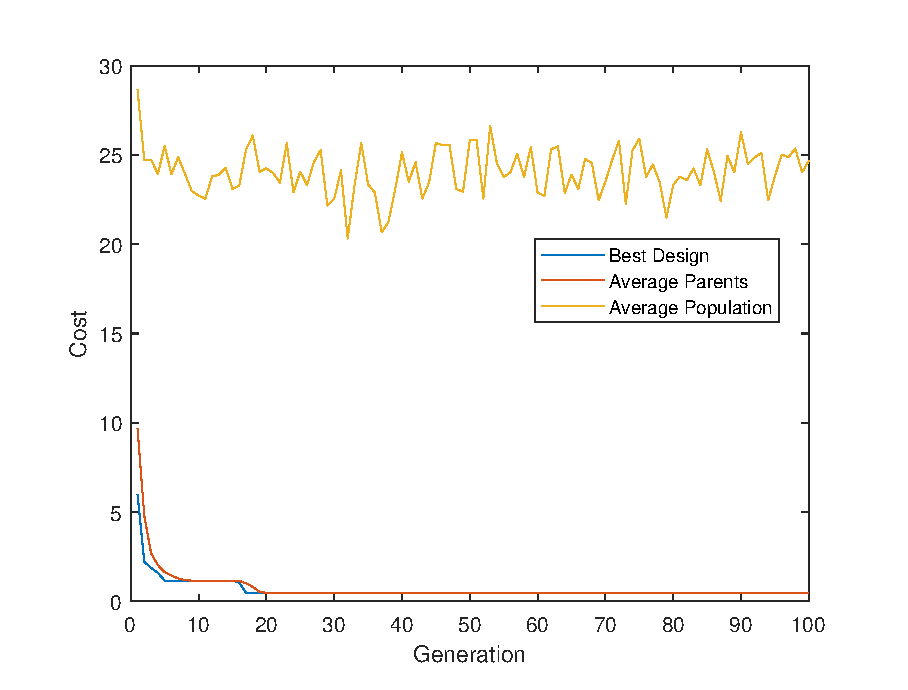
\includegraphics[width=0.75\linewidth]{part2_4.eps}
  \caption{Cost vs. Generation of the best design, average parents, and average overall population.}
  \end{nscenter}
\end{figure}

Both the cost of the best design and the average cost of the parents converges in a relatively small number of generations. The population cost only decreases in the first few generations, but then stays relatively constant, although noisy. This is because of the large population size relative to the number of parents and children. The random design parameters that make up 80 of the 100 designs in each population dominate the average cost for the population as a whole.

\section{Conclusion}
This project aimed to simulate a robotic 3D printer arm in two primary ways; one as a complete physical model with most significant phenomena accounted for, and two as a simplified physical model which enabled the use of numerical optimization as a means of finding parameters to produce a desired printed pattern.

Both models were formulated as a system of differential equations, and then solved using the Forward Euler method in the case of the complete model, or analytically in the case of the simplified model.

The models were then simulated for their duration using MATLAB, and a genetic algorithm was used to determine the optimal parameters for recreating a desired pattern with the simplified model. The complete model results are aligned with prior knowledge of dynamical systems, and the optimized simplified model produces a droplet pattern that is not visually discernible from that which was desired.


\section{Appendix}
Appendix is empty.



\end{document}